\documentclass{beamer}

\usepackage{graphicx}
\usepackage{amsmath}
\usepackage{natbib}
\usepackage{hyperref}
\usepackage{tikz}

\hypersetup{
colorlinks=true,
citecolor=blue,
linkcolor=blue,
urlcolor=blue
}

\bibliographystyle{apalike}

% Placeholder figure box
\newcommand{\imgplaceholder}[2]{
\fbox{
\begin{minipage}[c][#2][c]{#1}
\centering Placeholder for Figure
\end{minipage}
}
}

\title{Formation of Supermassive Black Holes}
\author{Krupa Pothiwala \& Liz Hayes}
\institute{Florida Institute of Technology}
\date{March 2026}

\begin{document}

\begin{frame}{}
\titlepage
\end{frame}

\begin{frame}
\frametitle{Outline}
\tableofcontents
\end{frame}

% =================================================
% Background
% =================================================

\section{Background Information}

\begin{frame}{Background Information}
\begin{itemize}

\item What are supermassive black holes?
\begin{itemize}
\item Black holes with masses above $100{,}000\,M_\odot$ \cite{Wikipedia2026}
\item Some reach several billion solar masses
\end{itemize}

\item Where are they found?
\begin{enumerate}
\item At the centers of most galaxies
\item Occasionally wandering through intergalactic space
\end{enumerate}

\item How are they formed?
\begin{itemize}
\item This is the question we are exploring
\end{itemize}

\end{itemize}
\end{frame}

% =================================================
% Source 1
% =================================================

\section{Formation of the First Supermassive Black Holes}

\usebackgroundtemplate{
\tikz[overlay,remember picture]
\node[opacity=0.65] at (current page.center)
{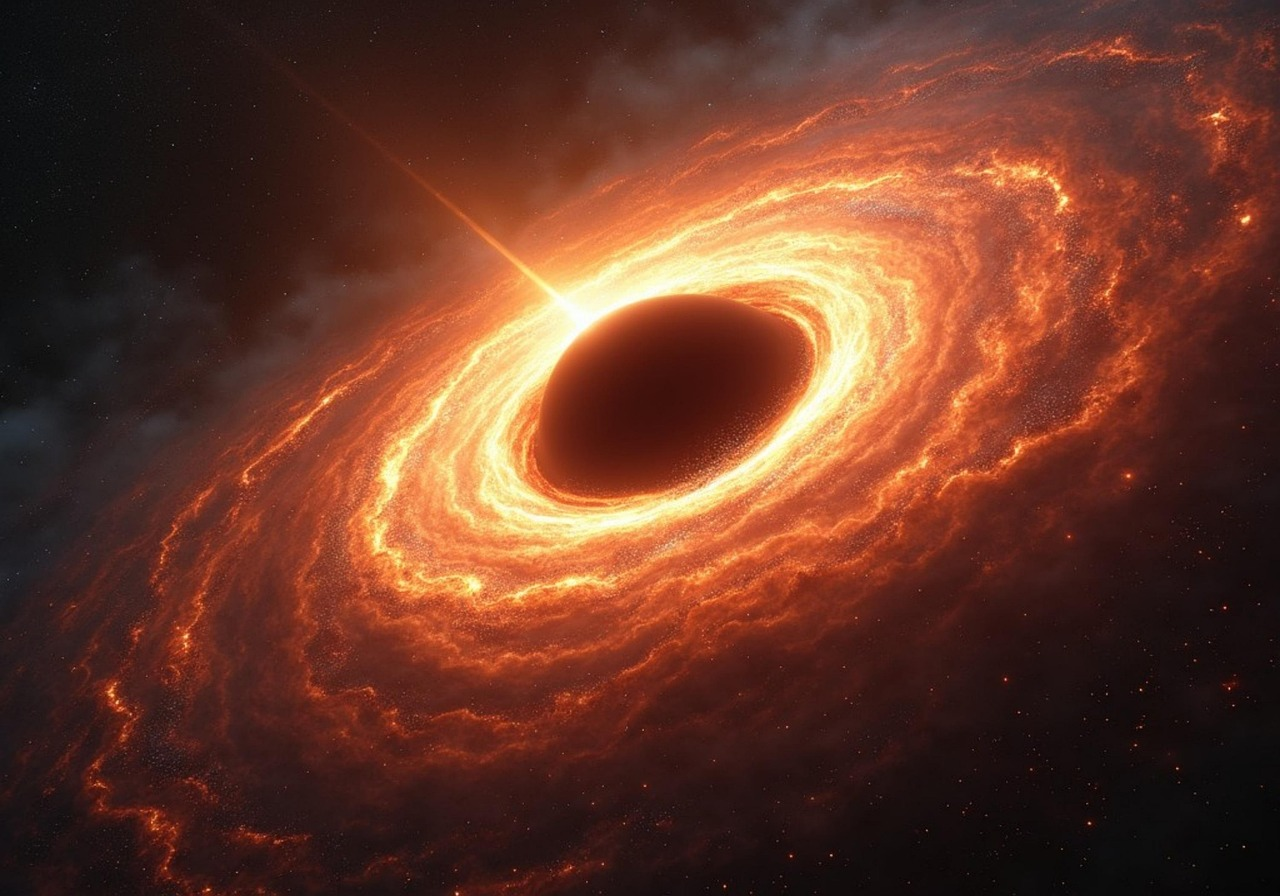
\includegraphics[width=\paperwidth,height=\paperheight]{black-hole.jpg}};
}

\begin{frame}{}
\vspace{1.2cm}
\begin{center}
\textbf{\textcolor{black}{Formation of the First Supermassive Black Holes}}
\end{center}
    \begin{tikzpicture}[remember picture, overlay]
    \node[anchor=south west, inner sep=6pt] at (current page.south west) {
        \tiny \textcolor{white}{Image: \href{https://www.archyde.com/early-universe-may-experience-dual-ionization-stages-with-supermassive-black-hole-formation-in-the-first-stage/}{Archyde -- SMBH: Echoes of the Universe’s First stars?}}
    };
    \end{tikzpicture}
\end{frame}

\usebackgroundtemplate{}

% -------------------------------------------------

\begin{frame}{Why Direct Collapse?}
\footnotesize

\begin{itemize}
\item Quasars are observed at redshift $z>6$, less than 1 billion years after the Big Bang
\item These quasars already host black holes with masses $\sim10^9\,M_\odot$
\item Stellar-mass seeds ($10$--$100\,M_\odot$) may not grow quickly enough
\item \cite{Bromm2003} explores whether gas clouds could collapse directly into massive seeds
\end{itemize}

\vspace{0.2cm}

\begin{center}
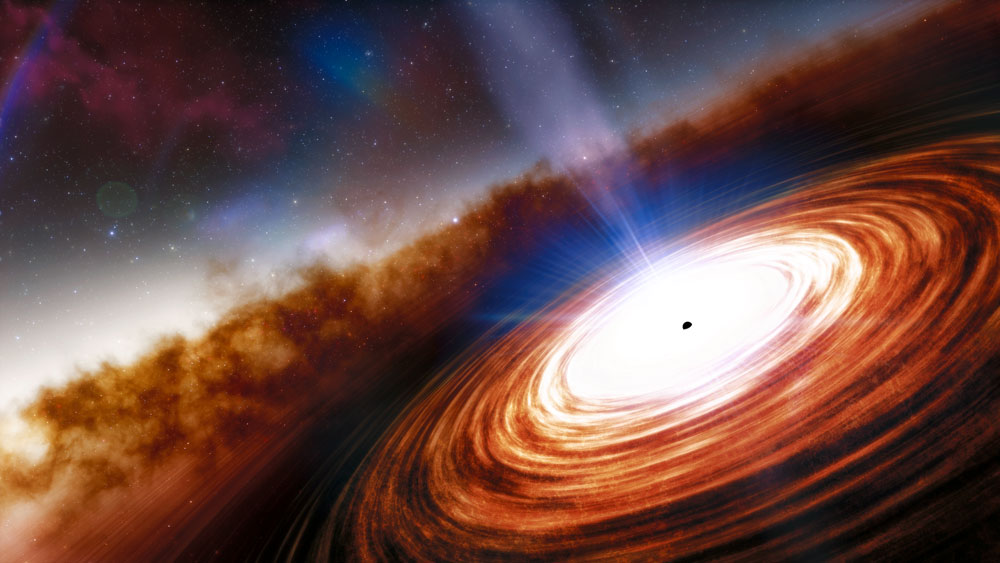
\includegraphics[width=0.72\textwidth,height=0.42\textheight,keepaspectratio]{Quasar.jpg}
\end{center}

\end{frame}

% -------------------------------------------------
\begin{frame}{Key Conditions for Direct Collapse}

\begin{center}
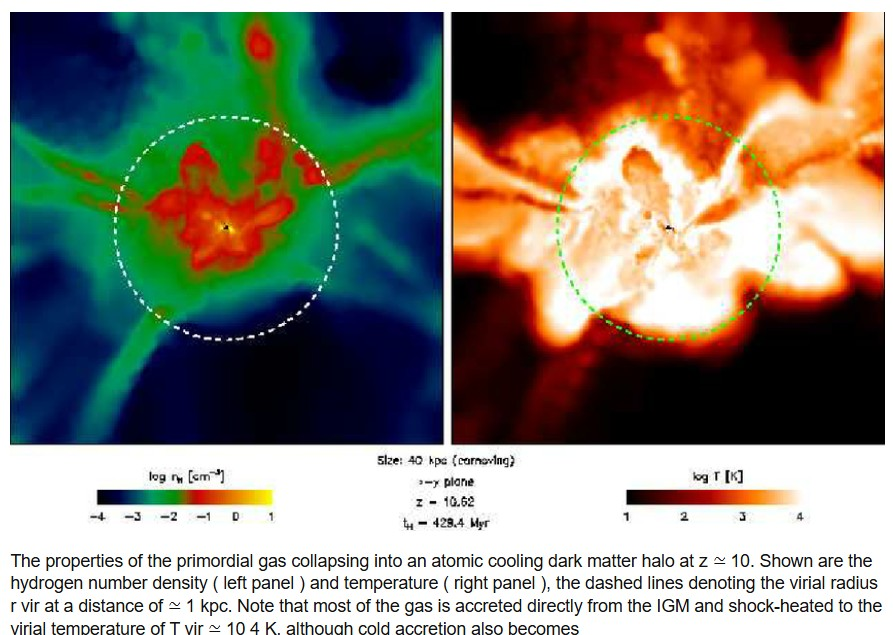
\includegraphics[width=0.78\textwidth,height=0.50\textheight,keepaspectratio]{Primordial Gas Collapse.jpg}
\end{center}

\vspace{0.25cm}

\footnotesize
\begin{itemize}
\item Gas must be nearly metal-free
\item Strong ultraviolet radiation destroys molecular hydrogen (H$_2$)
\item H$_2$ normally allows primordial gas to cool
\item Without H$_2$, gas stays hot ($\sim10^4$ K)
\item Hot gas prevents fragmentation into many stars
\item Gas collapses more smoothly toward the halo center
\end{itemize}

\end{frame}

\begin{frame}{Simulation Setup}
\footnotesize
\begin{columns}

\column{0.58\textwidth}

\begin{itemize}
\item Simulates collapse of a $\sim10^8\,M_\odot$ halo at $z\sim10$
\item Uses Smoothed Particle Hydrodynamics (SPH)
\item Tracks gas motion and cooling
\item Chemical network follows hydrogen and helium species
\item Compares cases with and without H$_2$ cooling
\end{itemize}

\column{0.38\textwidth}

    \begin{figure}
        \centering
        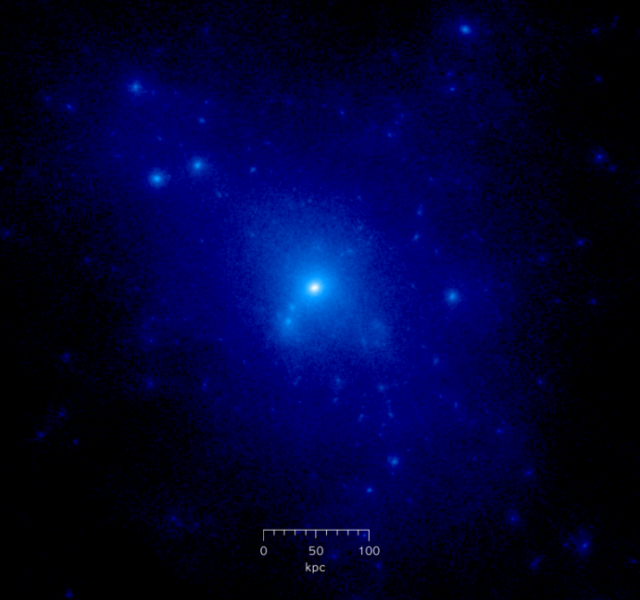
\includegraphics[width=\textwidth]{Dark_matter_halo.png}
        \caption{\tiny Simulated dark matter halo from a cosmological N-body simulation. Taken from \href{https://en.wikipedia.org/wiki/Dark_matter_halo}{Wikipedia}.}
    \end{figure}

\end{columns}
\end{frame}

% -------------------------------------------------

\begin{frame}{Main Result}
\footnotesize
\begin{columns}

\column{0.38\textwidth}

    \begin{figure}
        \centering
        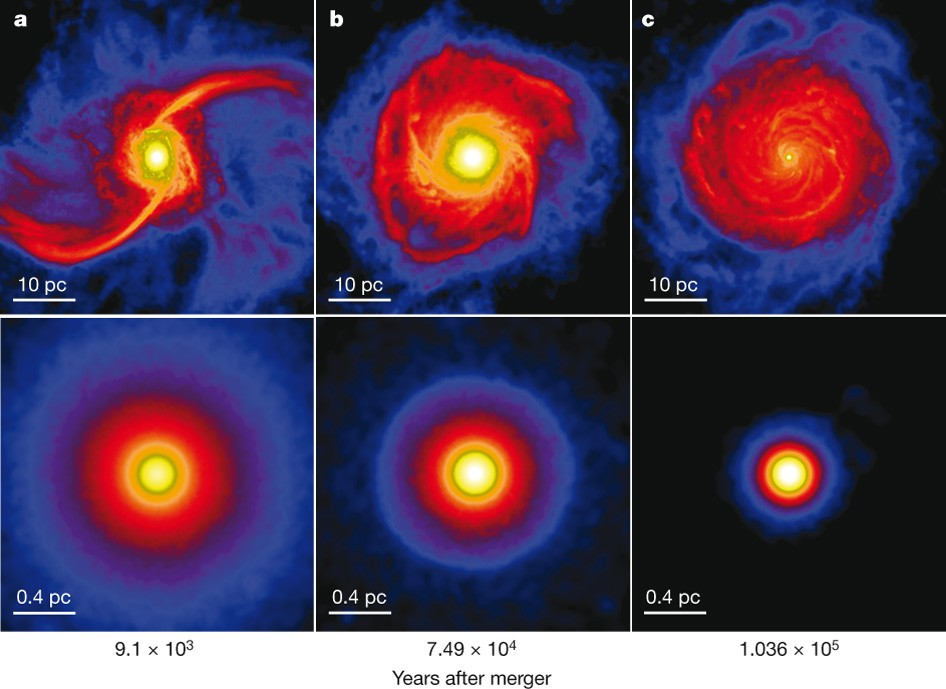
\includegraphics[width=\textwidth]{41586_2010_Article_BFnature09294_Fig1_HTML.jpg}
        \caption{\tiny Time evolution of the nuclear gas disk from its formation until the onset of central collapse. Taken from \href{https://www.nature.com/articles/nature09294}{Nature article}}
    \end{figure}

\column{0.58\textwidth}

\begin{itemize}
\item Without H$_2$ cooling, gas remains near $\sim10^4$ K
\item Fragmentation into normal stars is suppressed
\item Gas collapses toward the halo center
\item A central clump forms with mass $\sim10^6\,M_\odot$
\item More than 10\% of halo gas can collect in the nucleus
\end{itemize}

\end{columns}
\end{frame}

% -------------------------------------------------

\begin{frame}{Takeaways from Source 1}
\footnotesize
\begin{columns}

\column{0.58\textwidth}

\begin{itemize}
\item Direct collapse can form massive black hole seeds quickly
\item Typical seed masses are $\sim10^5$--$10^6\,M_\odot$
\item This helps explain quasars observed at $z>6$
\item Requires rare conditions:
\begin{itemize}
\item metal-free gas
\item strong UV radiation
\item massive halos
\end{itemize}
\end{itemize}

\column{0.38\textwidth}

  \begin{figure}
        \centering
        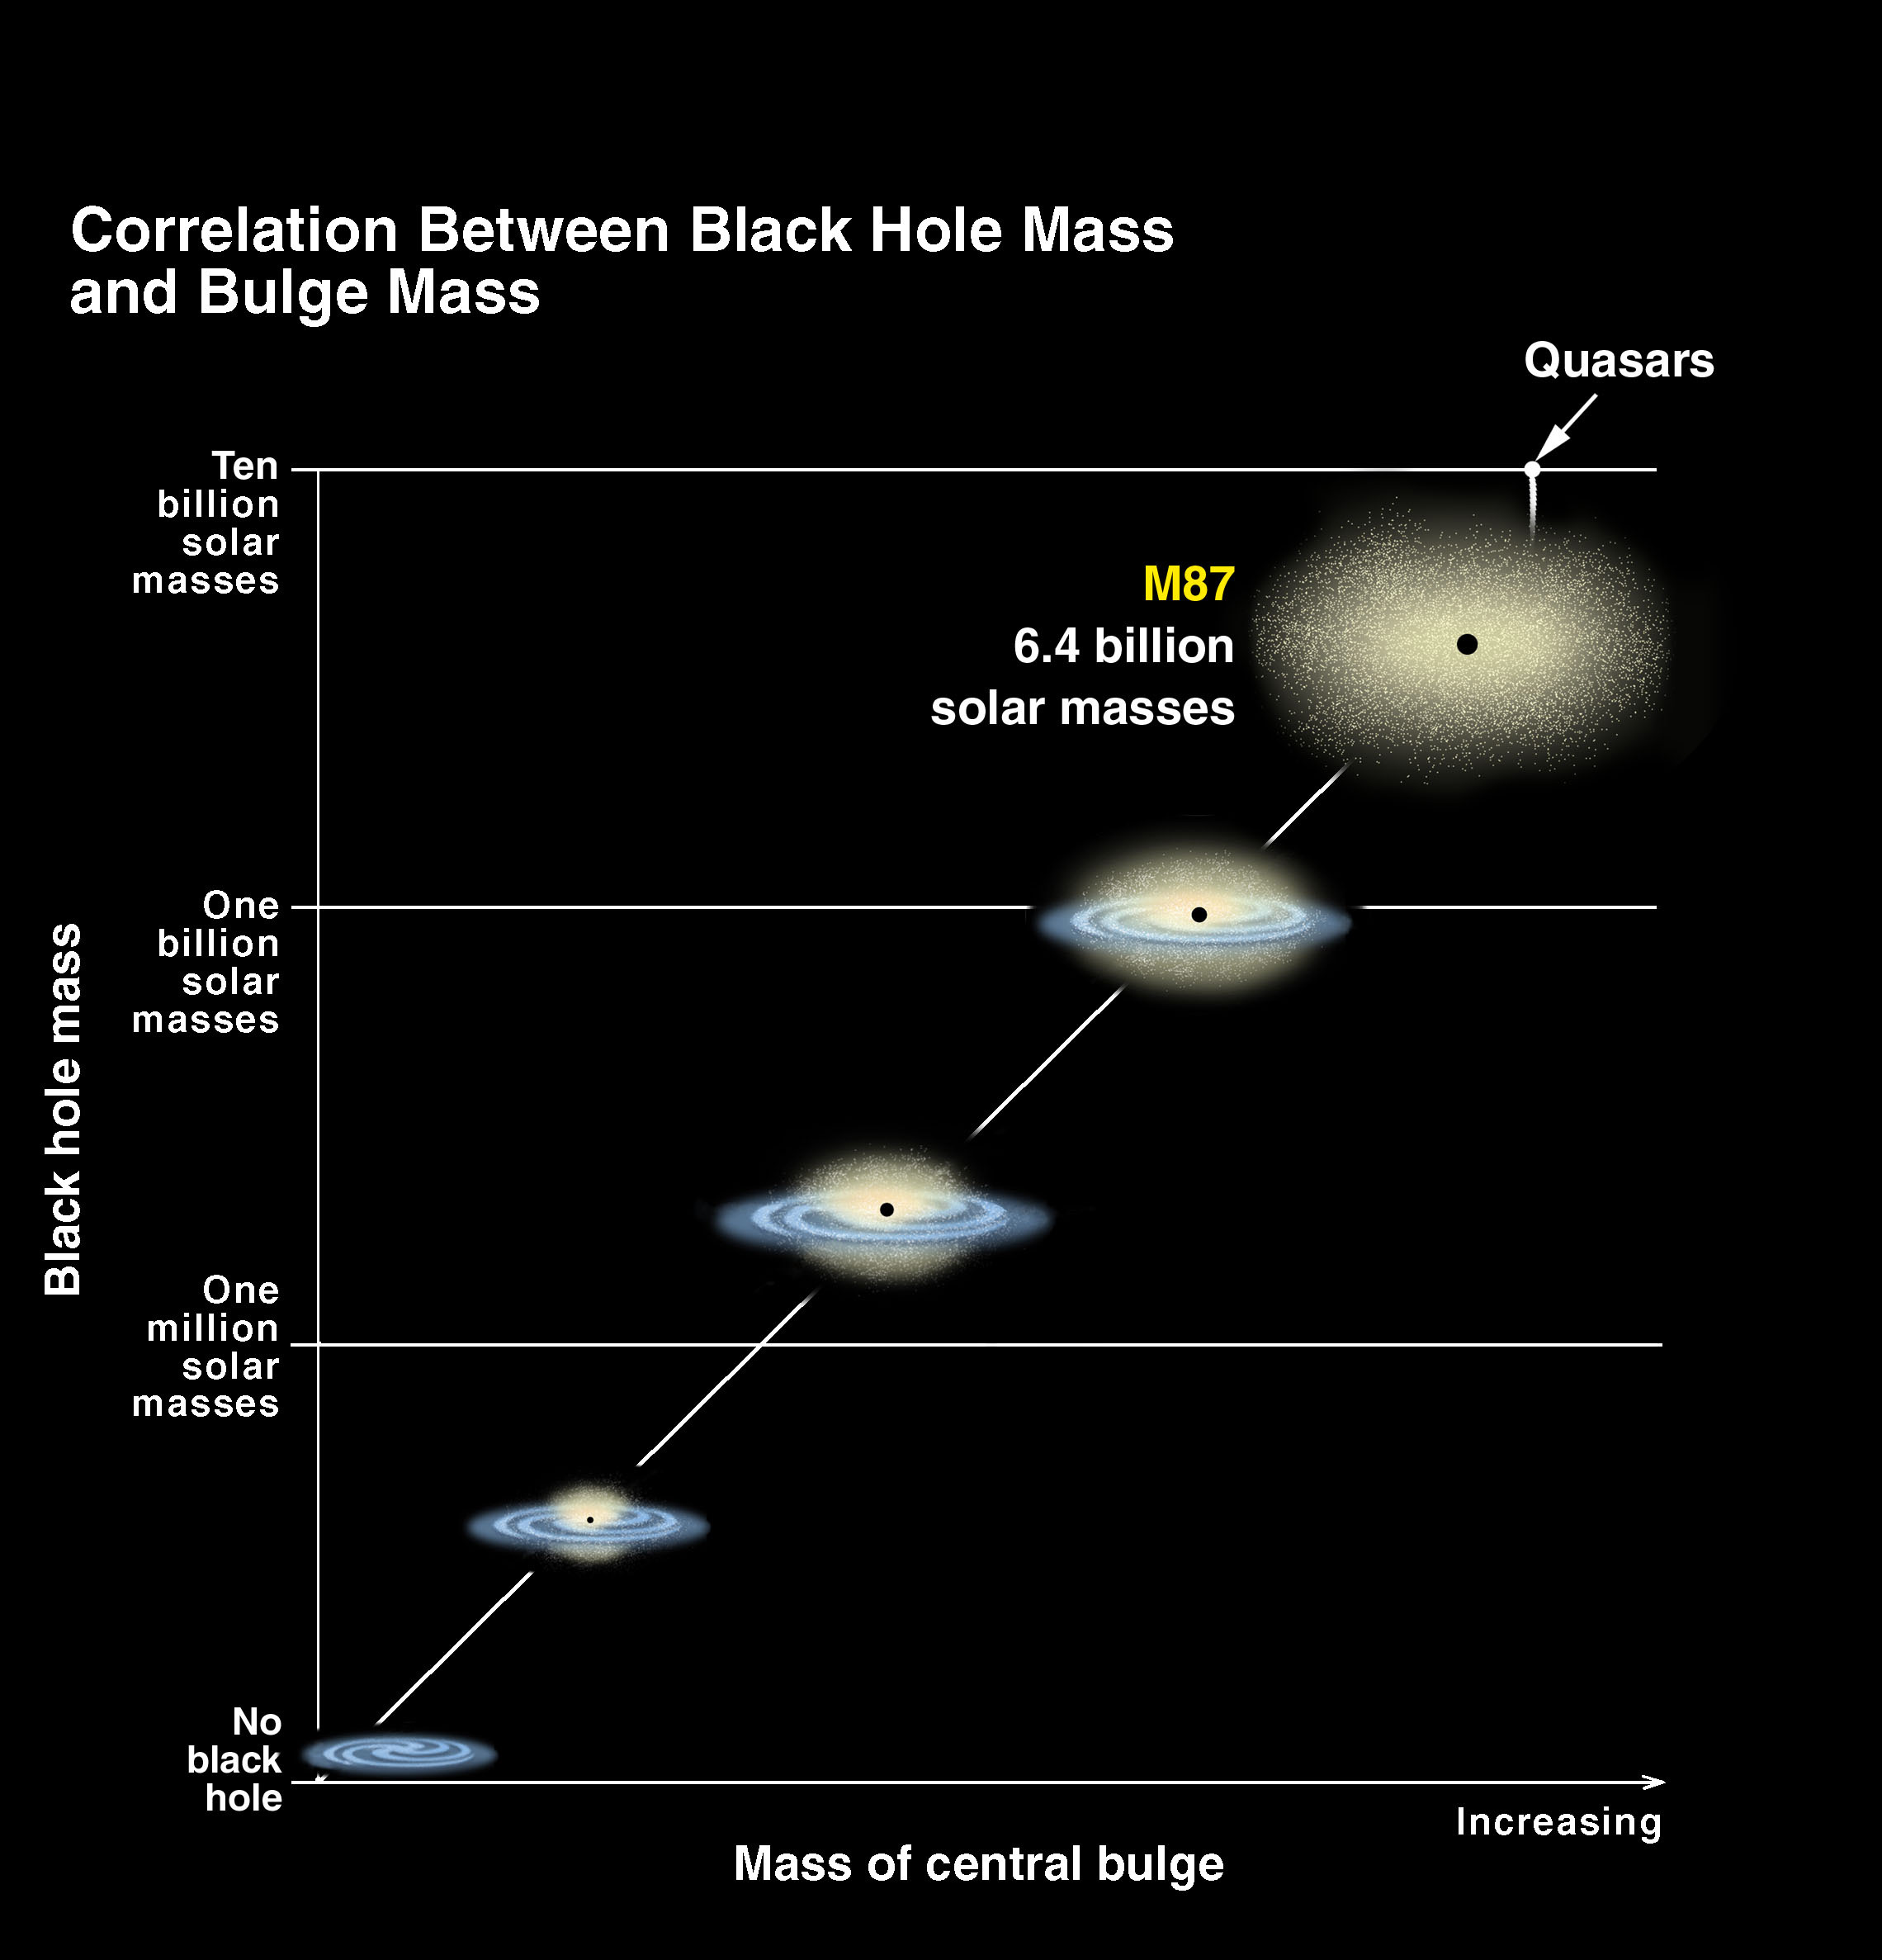
\includegraphics[width=\textwidth]{bhdiagram_1.jpg}
        \caption{\tiny The illustration shows the relationship between the mass of a galaxy's central black hole and the mass of its central bulge. Taken from \href{https://mcdonaldobservatory.org/news/gallery/black-hole-diagram}{The University of Texas McDonald Observatory}}
    \end{figure}

\end{columns}
\end{frame}

% =================================================
% Source 2
% =================================================

\section{Formation of SMBHs by Direct Collapse in Pregalactic Halos}

\usebackgroundtemplate{
\tikz[overlay,remember picture]
\node[opacity=0.60] at (current page.center)
{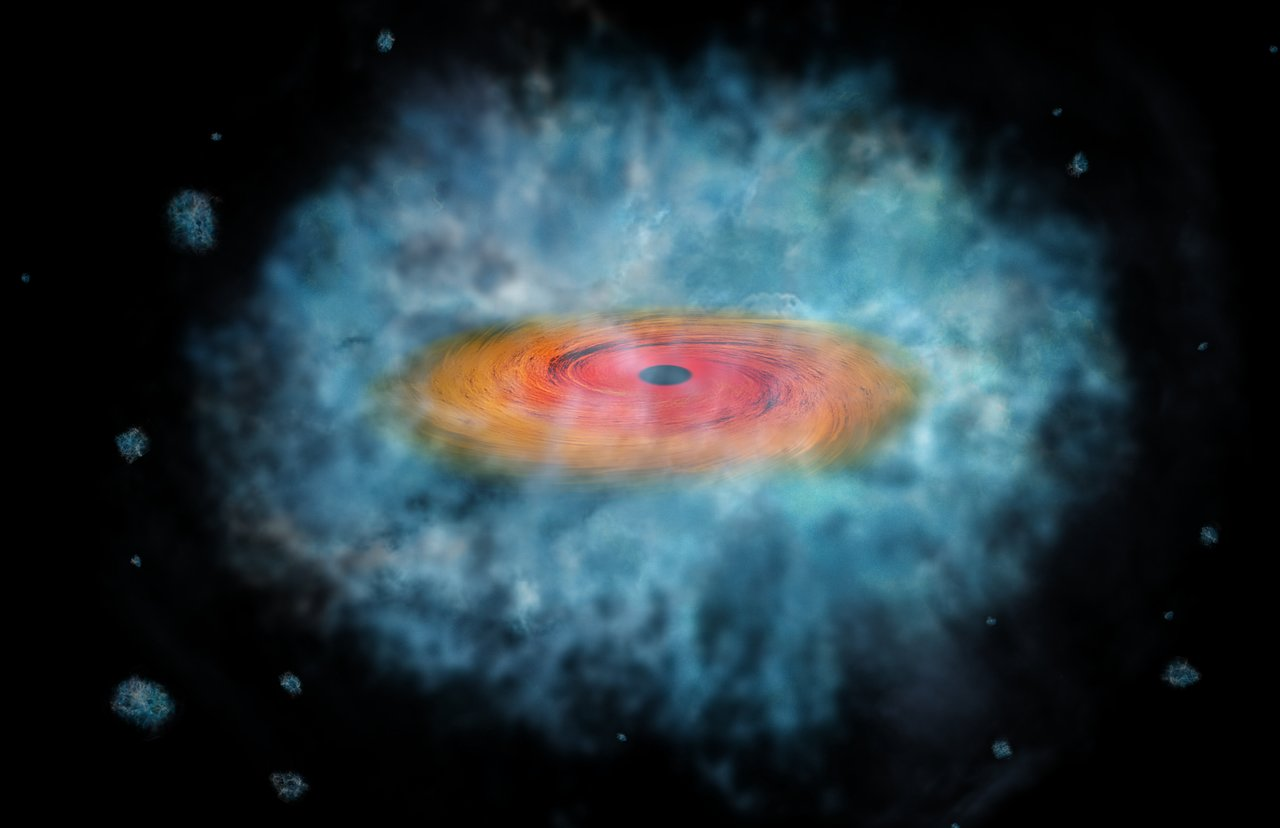
\includegraphics[width=\paperwidth,height=\paperheight]{Artist’s_impression_of_supermassive_black_hole_seed.jpg}};
}

\begin{frame}{}
\begin{center}
\textbf{\textcolor{black}{Formation of Supermassive Black Holes by Direct Collapse in Pregalactic Halos}}
\end{center}

\begin{tikzpicture}[remember picture, overlay]
    \node[anchor=south west, inner sep=6pt] at (current page.south west) {
        \tiny \textcolor{white}{Image: \href{https://en.wikipedia.org/wiki/Direct_collapse_black_hole}{Wikipedia -- Direct Collapse Black Hole}}
    };
\end{tikzpicture}
\end{frame}

\usebackgroundtemplate{}

% -------------------------------------------------

\begin{frame}{Formation directly in the nuclei of protogalaxies}
\begin{itemize}
\item How is it possible to generate a SMBH at $z \sim 6$?
\vspace{0.2cm}
\item \cite{Begelman2006} proposes that SMBHs form directly from gas in early halos
\vspace{0.2cm}
\item Halos with virial temperature $\sim10^4$ K allow atomic hydrogen cooling
\vspace{0.2cm}
\item Gas begins collapsing toward the halo center
\vspace{0.2cm}
\item Angular momentum must be removed for collapse to continue
\end{itemize}
\end{frame}

% -------------------------------------------------

\begin{frame}{Bars Within Bars}
\begin{itemize}
\item Self-gravitating gas clouds become bar-unstable.
\vspace{0.2cm}
\item Bars transfer angular momentum outward through gravitational and hydrodynamical torques causing the radius to shrink.
\vspace{0.2cm}
\item The bar instability causes the gas/mass to fall inward
\vspace{0.2cm}
\item For this to hold there needs to metal free has in order to avoid gas fragmentation
\end{itemize}
\end{frame}

% -------------------------------------------------

\begin{frame}{Quasi-Star}
\begin{columns}

\column{0.45\textwidth}

\begin{itemize}
\item Gas accumulates rapidly in the halo center
\item A massive object called a quasi-star forms
\item The envelope is supported by radiation pressure
\item Pressure decreases and causes core collapse
\item Rapid accretion allows fast black hole growth
\end{itemize}

\column{0.55\textwidth}

 \begin{figure}
            \centering
            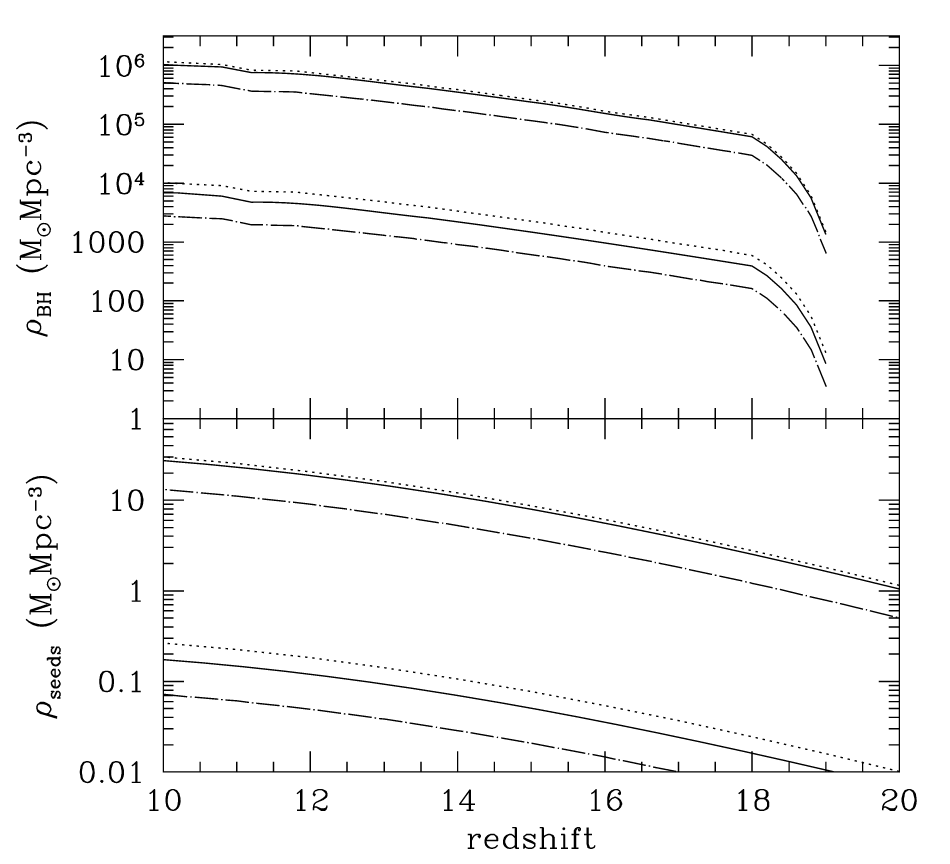
\includegraphics[width=\textwidth]{fig2.png}
            \caption{\small Comoving density of BH seeds (bottom) growing to $10^6\,M_\odot$ (top), from $z=20$ to $z=10$ \citep{Begelman2006}.}
        \end{figure}

\end{columns}
\end{frame}

% =================================================
% References
% =================================================

\section{SMBH formation via collisions in BH clusters}
%% Adding background picture
\usebackgroundtemplate{
    \tikz[overlay, remember picture]
        \node[opacity=0.60, at=(current page.center)] {
            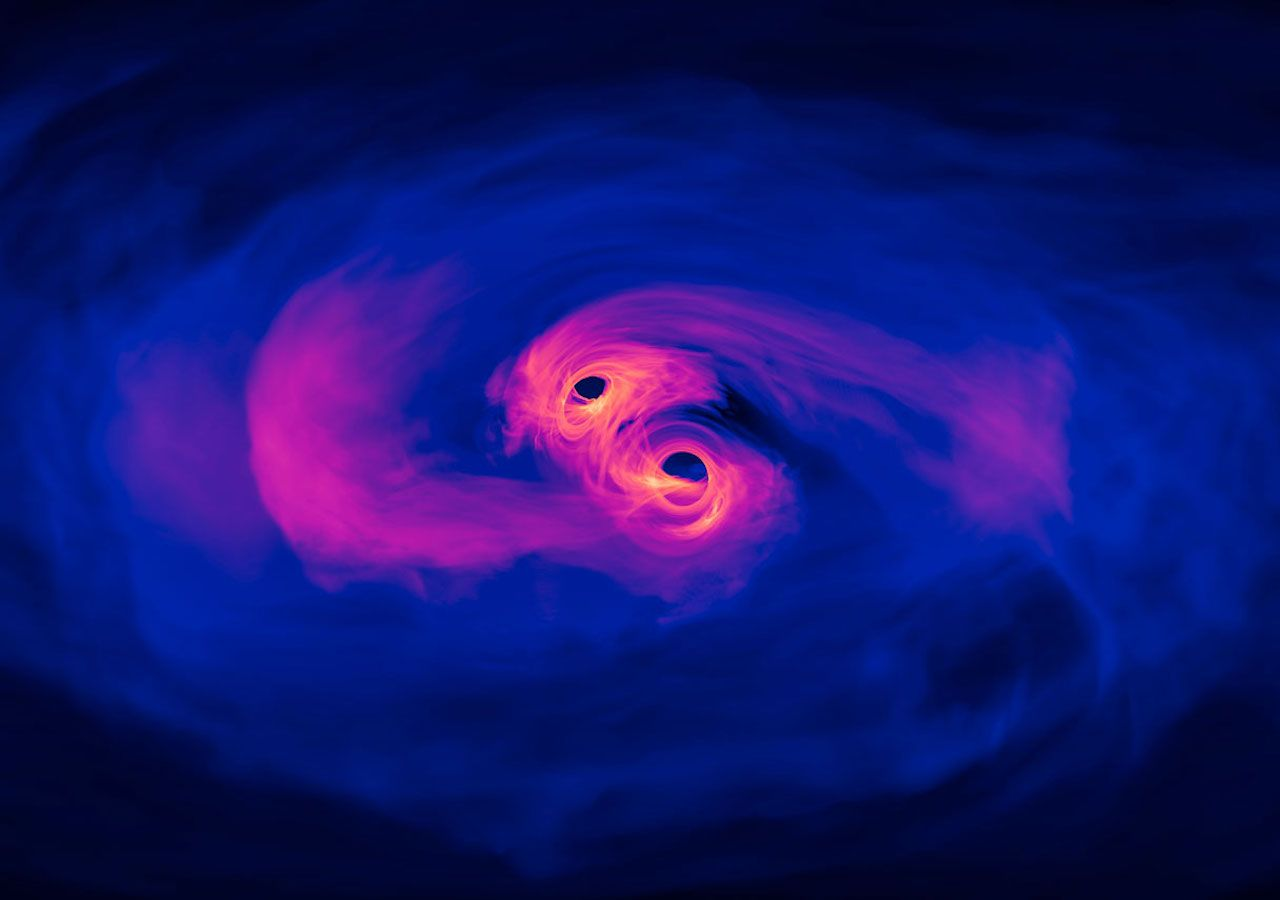
\includegraphics[width=\paperwidth, height=\paperheight]{Formation-of-supermassive-black-holes.jpg}
        };
}
\begin{frame}{}
    \begin{center}
        \textbf{\textcolor{black}{Supermassive Black Hole Formation via Collisions in Black Hole Clusters}}
    \end{center}
    
    \begin{tikzpicture}[remember picture, overlay]
    \node[anchor=south west, inner sep=6pt] at (current page.south west) {
        \tiny \textcolor{white}{Image: \href{https://animalia-life.club/qa/pictures/nasa-black-hole-merger-simulation}{Nasa Black Hole Merger Simulation}}
    };
    \end{tikzpicture}
\end{frame}

%% Resetting the background
\usebackgroundtemplate{}
\begin{frame}{Dense Cluster Formation}
    \begin{itemize}
        \item The universe is known to host Nuclear Star Clusters where SMBHs co-exist  \cite{Gaete2024}
        \item Fragmentation causes stars to be packed very close together this increases stellar density
        \item Due to high stellar density the cluster can undergo runaway core collapse, causing an intermediate-mass black hole ($\sim 10^{2-4}$ M$_\odot$)
        \item The BH could be surrounded by inflow of gas increasing the gravitational potential of the cluster. 
        \item As well as dynamical friction will increase the gravitational potential
    \end{itemize}
\end{frame}

\begin{frame}{Thought Experiment}
\begin{itemize}
    \item Consider a cluster made of stellar-mass black holes and stars
    \item The BH will start forming Binaries. These binaries are going to interact with other black holes. \textcolor{violet}{What do you think will happen?}
    %% The third black hole will recieve additional energy and it will be sling shotted away from the binary and the binary will harden aka get closer together.
    \item This causes the cluster to stabilize and not collapse in on itself
    \item This is how velocity dispersion holds off gravitational collapse
\end{itemize}
\vspace{0.2cm}
Eventually the binary gets close enough and starts radiating gravitational waves and merges into a single black hole increasing the average black hole mass in the cluster
\end{frame}

\begin{frame}{Forming a SMBH}
    \begin{columns}
    
        \column{0.5\textwidth}
        \begin{itemize}
            \item Since the binary merged the gravity overpower the velocity dispersion
            \item During this phase: density rises dramatically, encounter rates increase, and mergers become much more frequent.
            \item A runaway growth process begins where one black hole grows rapidly through repeated mergers. This produces a massive central black hole.
        \end{itemize}

        \column{0.5\textwidth}
        \begin{figure}
            \centering
            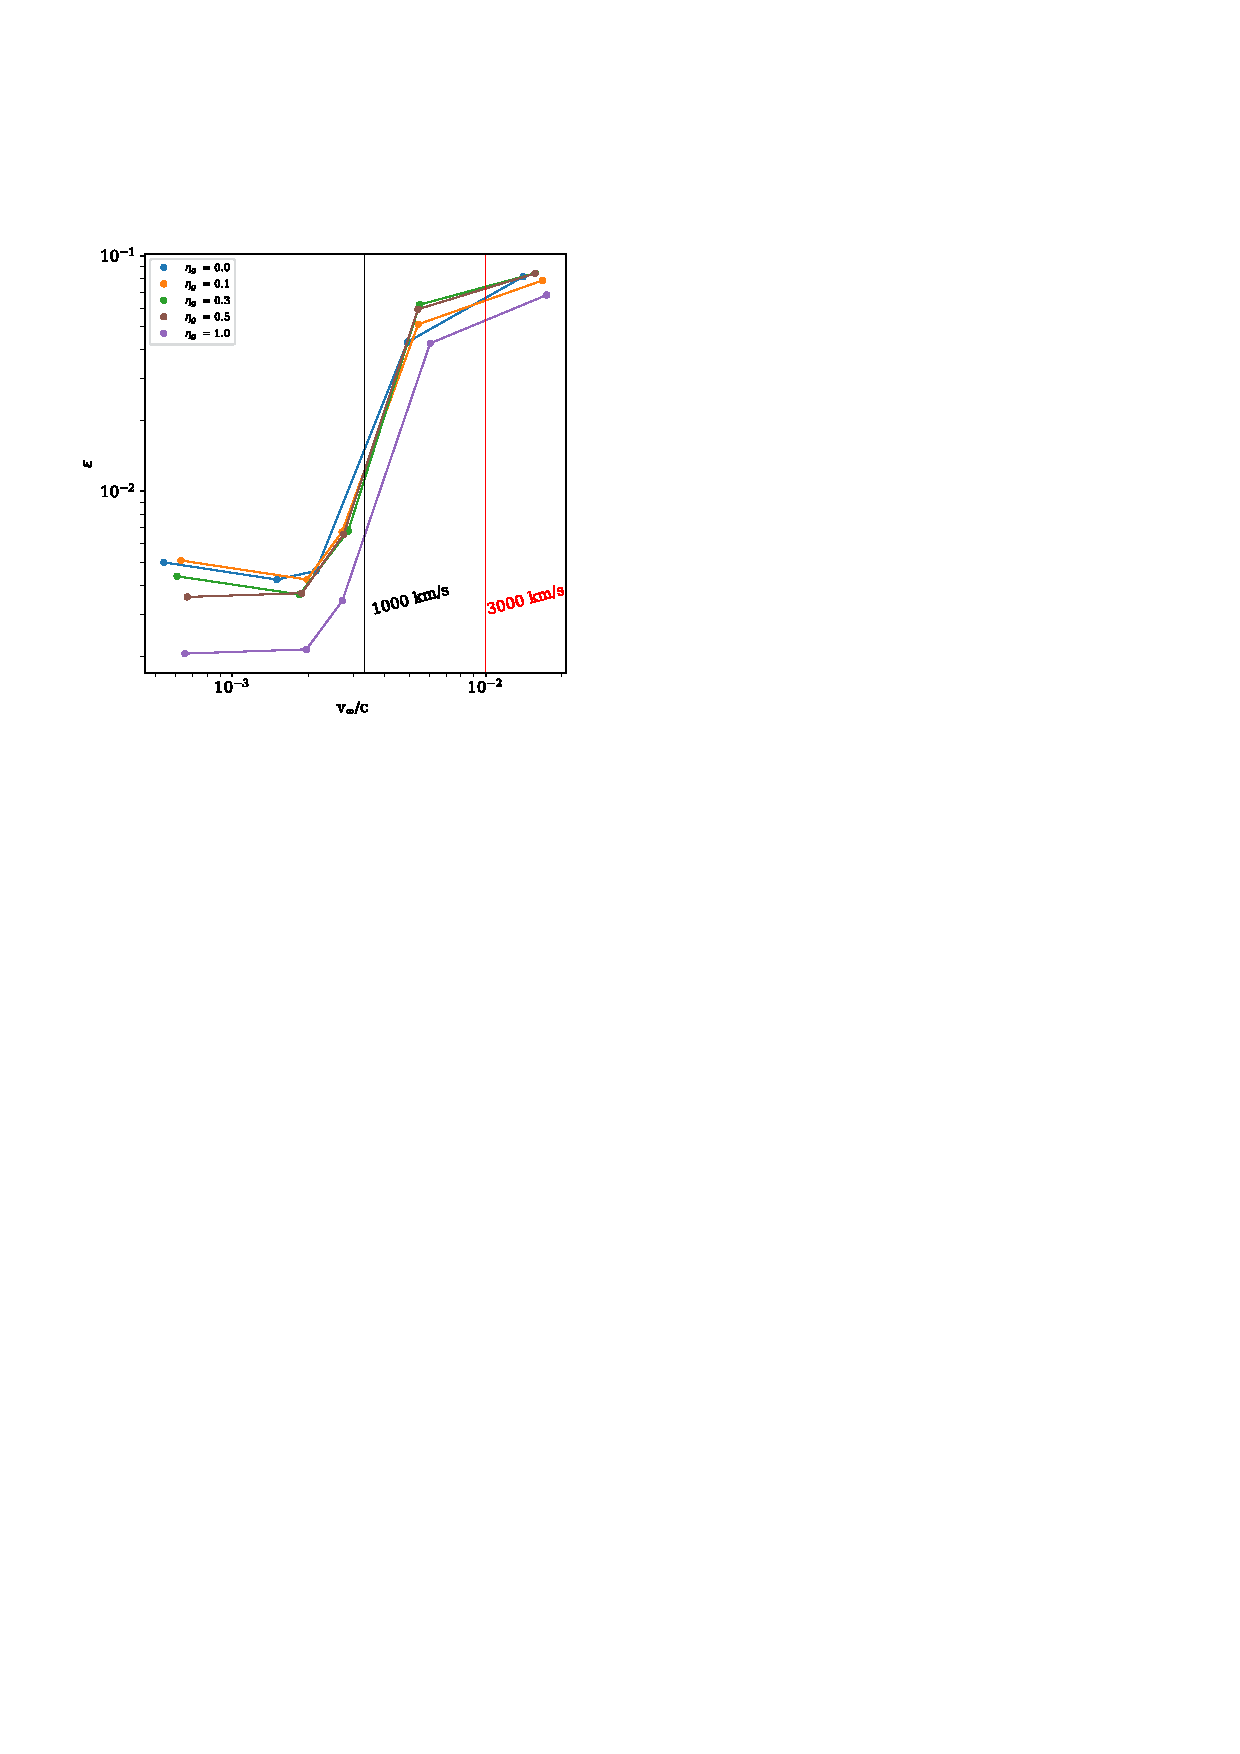
\includegraphics[width=\textwidth]{fig8.pdf}
            \caption{\small Formation efficiency of the most massive BH as a function of cluster velocity relative to the speed of light \citep{Gaete2024}.}
        \end{figure}
    %% The horizontal axis shows how fast the black holes are moving as a fraction of the speed of light — this is the "relativistic-ness" of the cluster 
    %% The vertical axis shows how efficient the merger process is — how much of the cluster's mass ends up in one big black hole seed
    \end{columns}
\end{frame}
\section{References}
\begin{frame}{References}
  \bibliography{references}

  
\end{frame}

\end{document}